\documentclass[../../main.tex]{subfiles}
\begin{document}
\section{Relations binaires et ordre}
\label{sec:relations_binaires_et_ordre}
Les relations binaires sont \textit{extrêmement} utilisées en informatique, raison du rappel. En effet, elles sont équivalentes (strictement le même objet) à la structure de \textit{graphe non enrichi}.

Une relation binaire entre les éléments de deux ensembles $A$ et $B$ est un ensemble d'associations entre $A$ et $B$, caractérisant les éléments qui sont ``en relation'' les uns avec les autres. La nature de la relation en question peut être très variée :
\begin{itemize}
	\item similarité entre les objets (comme $=$)
	\item hiérarchie entre un tout et ses parties (comme $\in$ ou son extension $\subseteq$)
	\item comparaison de grandeurs (comme $\leq$)
	\item antécédents et images d'une fonction
	\item dépendance entre deux évènements
	\item accessibilité d'un point d'arrivée depuis un point de départ ($\rightarrow$ en théorie des graphes)
\end{itemize}
Ces exemples parcourent plusieurs grands types de relations en mathématiques, à savoir les relations fonctionnelles, les relations d'équivalence et les relations d'ordre.

\subsection{Relation}
\definition{Relation}{
	Une \textit{relation} d'un ensemble $A$ dans un ensemble $B$ est définie par un ensemble de paires $\mathcal{R}\subseteq A\times B$. Si $(a, b)\in \mathcal{R}$, on dit que $a$ et $b$ sont ``mis en relation'' par $\mathcal{R}$ et on note $a\mathcal{R}b$. Si $A = B$, on dit que $\mathcal{R}$ est une relation \textit{homogène}.
}
Ce sous-ensemble de $A\times B$ définit le \textit{graphe} de $\mathcal{R}$ qui est noté $G_{\mathcal{R}}$\footnote{On peut aussi définir le graphe comme la relation, ce qui est équivalent. Il s'agit de la même chose}

On peut également voir une relation $\mathcal{R}$ de $A$ dans $B$ comme une application 
	$$\begin{array}{lclcl}\mathcal{R} & : & A & \rightarrow & \mathcal{P}(B) \\
& & a & \mapsto & \{b\in B\ |\ (a, b)\in \mathcal{R}\}
\end{array}$$
\textbf{Exemple :} si  $A = \{0, 1, 2, 3\}$, on peut représenter la relation homogène
$$\begin{array}{lclcl}\mathcal{R} & : & A & \rightarrow & \mathcal{P}(A) \\
& & a & \mapsto & \{a'\in A\ |\ a'\leq a\}
\end{array}$$
qui à chaque élément de $A$ associe les éléments qui lui sont inférieures par le graphe $G_{\mathcal{R}}$ :
\begin{center}
	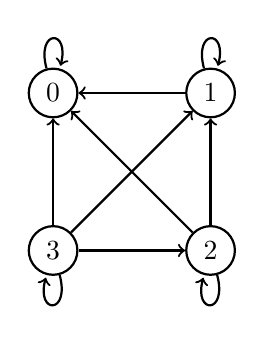
\begin{tikzpicture}[node distance={20mm}, thick, main/.style = {draw, circle}, auto=left] 
	% Sommets :
	\node[main] (0) {0}; 
	\node[main] (1) [right of=0] {1};
	\node[main] (2) [below of=1] {2};
	\node[main] (3) [left of=2] {3};
	% Arêtes
	\path
		(0) edge[loop above] (0)
		(1) edge[loop above] (1)
		(2) edge[loop below] (2)
		(3) edge[loop below] (3)
		(1) edge[->] (0)
		(2) edge[->] (0)
		(3) edge[->] (0)
		(2) edge[->] (1)
		(3) edge[->] (2)
		(3) edge[->] (1);
	\end{tikzpicture} 
	\captionof{figure}{Graphe de $G_{\mathcal{R}}$\label{graph:ex_relation}}
\end{center}
Voir une relation de $A$ dans $B$ comme une application de $A$ dans $\mathcal{P}(B)$ permet de définir le \textit{domaine} et l'\textit{image} de la relation :
\definition{Domaine et image d'une relation}{
	Soit $\mathcal{R} : A\rightarrow \mathcal{P}(B)$ une relation de $A$ dans $B$. \\

	L'image de $\mathcal{R}$ est définie par :
	$$
	\begin{array}{lcl}\rm{Im}(\mathcal{R}) & = & \{b\in B\ |\ a\mathcal{R}b\} \\
	& = & \{b\in B\ |\ \exists a\in A / b\in \mathcal{R}(a)\} \\
	\end{array}
	$$
	Le domaine de $\mathcal{R}$ est  défini par :
	$$
	\begin{array}{lcl}\rm{Dom}(\mathcal{R}) & = & \{a\in A\ |\ \exists b\in B, a\mathcal{R}b\} \\
	& = & \{a\in A\ |\ \mathcal{R}(a)\neq \emptyset\} \\
	\end{array}
	$$
}
\begin{center}
	\includesvg[width=0.5\textwidth]{relation}
	\captionof{figure}{Graphe d'une relation}
\end{center}
On en déduit la relation de $B$ dans $A$ inverse de $\mathcal{R}$, noté $\mathcal{R}^{-1}$, telle que :
$$\begin{array}{lclcl}\mathcal{R} & : & B & \rightarrow & \mathcal{P}(A) \\
& & b & \mapsto & \{a\in A\ |\ (a, b)\in \mathcal{R}\}
\end{array}$$
c'est-à-dire telle que $b\mathcal{R}^{-1}a \Leftrightarrow a\mathcal{R}b$.

On a immédiatement :
\begin{itemize}
	\item $G_{\mathcal{R}^{-1}} = G_{\mathcal{R}}^{t}$
	\item $\rm{Im}(\mathcal{R}^{-1}) = \rm{Dom}(\mathcal{R})$
	\item $\rm{Dom}(\mathcal{R}^{-1}) = \rm{Im}(\mathcal{R})$
\end{itemize}
\definition{Propriétés standards des relations homogènes}{
	Soit $E$ un ensemble et $\mathcal{R}$ une relation homogène sur $E$ (\textit{i.e.} $\mathcal{R}\subseteq E\times E$). \\

	On dit que $\mathcal{R}$ est :
	\begin{itemize}
		\item \textit{réflexive} si et seulement si $\forall e\in E, e\mathcal{R}e$
		\item \textit{transitive} si et seulement si $\forall e, f, g\in E, e\mathcal{R}f\text{ et }f\mathcal{R}g \Rightarrow e\mathcal{R}g$
		\item \textit{symétrique} si et seulement si $\forall e, f\in E, e\mathcal{R}f \Rightarrow f\mathcal{R}e$ (\textit{i.e.} $\mathcal{R} = \mathcal{R}^{-1}$)
		\item \textit{antisymétrique} si et seulement si $\forall e, f\in E, e\mathcal{R}f\text{ et }f\mathcal{R}e\Rightarrow e = f$
	\end{itemize}
}
\subsection{Relations d'équivalence}
\definition{Relation d'équivalence}{
	Une relation \textit{d'équivalence} $\mathcal{R}$ de $E$ dans $E$ est une relation réflexive, transitive et symétrique.
}
\textbf{Exemple :} les relations homogènes sur $\mathbb{Z}$ définies pour $n\in\mathbb{N}\setminus \{0\}$ par :
$$
\mathcal{R}_n = \{(a, b)\in \mathbb{Z}^2\ |\ \exists k\in\mathbb{Z}, a - b = nk\}
$$
sont des relations d'équivalences totales sur $\mathbb{N}$.
\definition{Classes d'équivalences et quotient}{
	Soit $E$ un ensemble et $\mathcal{R}$ une relation d'équivalence sur $E$. La \textit{classe d'équivalence} d'un élément $e\in E$ est :
	$$
	[e]_{\mathcal{R}} = \{e'\in E\ |\ e'\mathcal{R}e\}
	$$
	L'ensemble des classes d'équivalences de $E$ par $\mathcal{R}$ appelé \textit{quotient} de $E$ par $\mathcal{R}$ :
	$$
	E/\mathcal{R} = \{[e]_{\mathcal{R}}\subseteq E\ |\ e\in E\}
	$$
}
\proposition{Propriétés des classes d'équivalences} Si $\mathcal{R}$ est une relation d'équivalence sur un ensemble $E$, alors :
\begin{enumerate}
	\item tout élément $e\in E$ appartient à au moins une classe d'équivalence
	\item $a\mathcal{R}b \Leftrightarrow [a]_{\mathcal{R}} = [b]_{\mathcal{R}}$
\end{enumerate}
On en déduit que les classes d'équivalences de $E$ par $\mathcal{R}$ forment une partition de $E$ :
$$
E = \displaystyle\bigsqcup_{C\in E/\mathcal{R}}C
$$
\textbf{Exemple (suite) :} Soit $n\in\mathbb{N}$. Les classes d'équivalences d'une relation $\mathcal{R}_{n}$ telle que définie plus haut sont les restes possibles par la division euclidienne par $n$, c'est-à-dire :
$$
\mathbb{Z}/\mathcal{R}_n = \mathbb{Z}/n\mathbb{Z} = \{\dot{1}, \dots, \dot{n}\} \text{ (où on note $\dot{k} = [k]_{\mathcal{R}_n}$)}
$$
Ce quotient sera utilisé au chapitre \ref{cha:les_donn_es} pour l'interprétation entière signée des mots binaires.

\subsection{Clôture}
Il est parfois pratique de décrire une relation homogène en ne donnant qu’une
partie de son graphe, mais en précisant que la relation doit être complétée pour
avoir une ou plusieurs des propriétés standards de ce type de relation. Cette complétion de la relation est appelée sa \textit{clôture}.
\definition{Clôture}{
	Soit $\mathcal{R}$ une relation homogène sur un ensemble $E$. La \textit{clôture transitive} (resp. \textit{réflexive}, \textit{symétrique}) est la plus petite relation homogène sur $E$ qui :
	\begin{itemize}
		\item contient $\mathcal{R}$
		\item est transitive (resp. réflexive, symétrique).
	\end{itemize}
	On note souvent $\mathcal{R}^{\star}$ la clôture transitive de $\mathcal{R}$
}
\proposition{La clôture transitive est l'accessibilité} Soit $\rightarrow$ une relation homogène sur $E$ et $\rightarrow^\star$ sa clôture transitive. Alors :
$$\forall (e,f)\in E^2, e\rightarrow^\star f \Leftrightarrow \exists e_0, \dots, e_n\in E, e = e_0 \text{ et } f = e_n\text{ et } \forall i < n, e_i\rightarrow e_{i+1}$$
\textbf{Démonstration :} l'énoncé à droite de $\Leftrightarrow$ définit une relation $\beta$ transitive qui contient $\rightarrow$ (puisque $\rightarrow^\star$ est la plus petite qui contient $\rightarrow$) et contenue dans toutes les relations transitives qui contiennent $\rightarrow$. Donc $\beta = \rightarrow^\star$

\textbf{Interprétation :} si la relation $\mathcal{R}$ (noté $\rightarrow$ dans la proposition) permet de se déplacer d'un élément $e$ vers un autre, la clôture transitive $\mathcal{R}^\star$ représente les éléments accessibles depuis $e$ par déplacements successifs dans $\mathcal{R}$.

\textbf{Exemple :} considérons une relation représentée par le graphe :
\begin{center}
	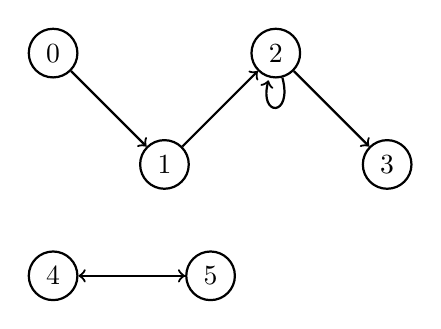
\begin{tikzpicture}[node distance={20mm}, thick, main/.style = {draw, circle}, auto=left] 
	% Sommets :
	\node[main] (0) {0}; 
	\node[main] (1) [below right of=0] {1};
	\node[main] (2) [above right of=1] {2};
	\node[main] (3) [below right of=2] {3};
	\node[main] (4) [below left of=1] {4};
	\node[main] (5) [right of=4] {5};
	% Arêtes
	\path
		(2) edge[loop below] (2)
		(0) edge[->] (1)
		(1) edge[->] (2)
		(2) edge[->] (3)
		(4) edge[->] (5)
		(5) edge[->] (4);
	\end{tikzpicture}
\end{center}
Les clôtures réflexive et transitive de cette relation sont représentées par les deux graphes suivant :
\begin{minipage}{0.32\textwidth}
	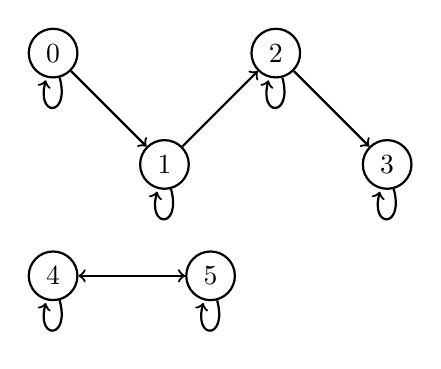
\begin{tikzpicture}[node distance={20mm}, thick, main/.style = {draw, circle}, auto=left] 
	% Sommets :
	\node[main] (0) {0}; 
	\node[main] (1) [below right of=0] {1};
	\node[main] (2) [above right of=1] {2};
	\node[main] (3) [below right of=2] {3};
	\node[main] (4) [below left of=1] {4};
	\node[main] (5) [right of=4] {5};
	% Arêtes
	\path
		(0) edge[loop below] (0)
		(1) edge[loop below] (1)
		(2) edge[loop below] (2)
		(3) edge[loop below] (3)
		(4) edge[loop below] (4)
		(5) edge[loop below] (5)
		(0) edge[->] (1)
		(1) edge[->] (2)
		(2) edge[->] (3)
		(4) edge[->] (5)
		(5) edge[->] (4);
	\end{tikzpicture}
	\begin{center}
	\captionof{figure}{Graphe \\de la clôture réflexive}
	\end{center}
\end{minipage}
\begin{minipage}{0.32\textwidth}
	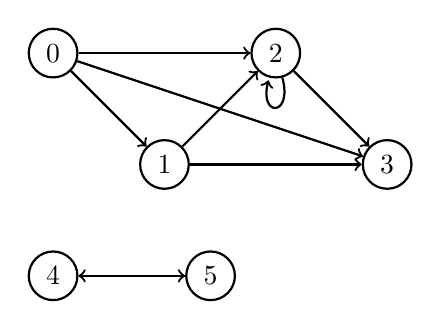
\begin{tikzpicture}[node distance={20mm}, thick, main/.style = {draw, circle}, auto=left] 
	% Sommets :
	\node[main] (0) {0}; 
	\node[main] (1) [below right of=0] {1};
	\node[main] (2) [above right of=1] {2};
	\node[main] (3) [below right of=2] {3};
	\node[main] (4) [below left of=1] {4};
	\node[main] (5) [right of=4] {5};
	% Arêtes
	\path
		(2) edge[loop below] (2)
		(0) edge[->] (1)
		(0) edge[->] (2)
		(0) edge[->] (3)
		(1) edge[->] (3)
		(1) edge[->] (2)
		(2) edge[->] (3)
		(4) edge[->] (5)
		(5) edge[->] (4);
	\end{tikzpicture}
	\begin{center}
	\captionof{figure}{Graphe \\de la clôture transitive}
	\end{center}
\end{minipage}
\begin{minipage}{0.32\textwidth}
	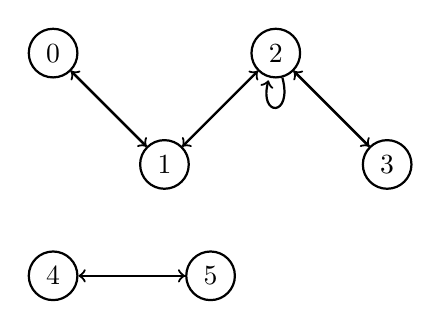
\begin{tikzpicture}[node distance={20mm}, thick, main/.style = {draw, circle}, auto=left] 
	% Sommets :
	\node[main] (0) {0}; 
	\node[main] (1) [below right of=0] {1};
	\node[main] (2) [above right of=1] {2};
	\node[main] (3) [below right of=2] {3};
	\node[main] (4) [below left of=1] {4};
	\node[main] (5) [right of=4] {5};
	% Arêtes
	\path
		(2) edge[loop below] (2)
		(0) edge[->] (1)
		(1) edge[->] (0)
		(1) edge[->] (2)
		(2) edge[->] (1)
		(2) edge[->] (3)
		(3) edge[->] (2)
		(4) edge[->] (5)
		(5) edge[->] (4);
	\end{tikzpicture}
	\begin{center}
	\captionof{figure}{Graphe \\de la clôture symétrique}
	\end{center}
\end{minipage}

L'\textit{union des arêtes} de ces trois graphes donne la clôture réflexive-transitive-symétrique du graphe, qui est donc une relation d'équivalence dont on voit bien les deux classes :
$$
\{0, 1, 2, 3, 4, 5\}/\mathcal{R^=} = \{[0]_{\mathcal{R}^=}, [4]_{\mathcal{R}^=}\}
$$
\subsection{Relations d'ordre}
\definition{Relation d'ordre}{
	Une relation \textit{d'ordre} $\mathcal{R}$ de $E$ dans $E$ est une relation réflexive, transitive et anti-symétrique. \\
	On appelle plus simplement une relation d'ordre un \textit{ordre}. \\

	Un ordre $\mathcal{R}$ est dit \textit{total} si $\forall e, f\in E, e\mathcal{R}f\text{ ou }f\mathcal{R}e$. C'est-à-dire que tout couple d'éléments peut être comparé. L'ordre est dit \textit{partiel} sinon. \\

	Soit $\leq$ est un ordre sur $E$. On appelle \textit{ordre strict associé à $\leq$} la relation $<$ telle que :
	$$\forall e, f\in E, e < f\Leftrightarrow e\leq f\text{ et }e\neq f$$
}
\definition{Bornes par un ordre}{
	Soit $\leq$ un ordre sur un ensemble $E$. Soit $P\subseteq E$ une partie de $E$.

	$e\in E$ est un \textit{minorant} (resp. \textit{majorant}) de $P$ si pour tout $p\in P$, $e\leq p$ (resp. $p\leq e$). Un minorant $e$ de $P$ est un \textit{minimum} (resp. \textit{maximum}) de $P$ si $e\in P$.
}
\definition{Ensembles bien ordonnés} {
	Un ensemble $E$ muni d'un ordre total $\leq$ est dit \textit{bien ordonné} si toute partie $P\subseteq E$ admet un minimum. On dit aussi que $\leq$ est un \textit{bon ordre} sur $E$.
}
\proposition{Descente infinie} Soit un ordre total $\leq$ sur un ensemble $E$. Les phrases suivantes sont équivalentes :
\begin{enumerate}
	\item $\leq$ est un bon ordre
	\item toute suite décroissante d'éléments de $E$ est constante à partir d'un certain rang
\end{enumerate}

\textbf{Démonstration :}
\begin{itemize}
	\item $(\Rightarrow)$ Supposons que $\leq$ est un bon ordre. Soit $s:\mathbb{N}\rightarrow E$ une suite décroissante d'éléments de $E$. Comme $\leq$ est un bon ordre, $\rm{Im}(s)$ admet un minimum. Il existe donc $N\in\mathbb{N}$ tel que pour tout $n\in\mathbb{N}, s(N) \leq s(n)$. Par décroissance de $s$, pour tout $n\geq N$, on a $s(n) \leq s(N)$ donc $s(n) = s(N)$ par antisymétrie.
	\item $(\Leftarrow)$ Supposons que $\leq$ n'est pas un bon ordre. Il existe donc une partie $P\subseteq E$ qui n'admet pas de minimum. Pour tout élément $p\in P$, il existe donc $p'\in P$ tel que $p'< p$ (sinon, $p$ est un minimum de $P$ car $\leq$ est total). On construit alors une suite $s:\mathbb{N}\rightarrow P$ telle que $s_0\in P$ et pour tout $n\geq 0$, $s_{n+1} = s_n'$ est tel que $s_{n+1}< s_n$. Cette suite est décroissante et jamais constante.
\end{itemize}
\section{Induction structurelle}
\label{sec:induction_structurelle}
\subsection{Principe sur un exemple}
La récurrence permet de construire des ensembles par répétition, itération, de règles simples. Par exemple, la suite d'éléments suivante $f : \mathbb{N} \rightarrow \mathbb{N}$ peut être définie par la récurrence suivante :
$$
\forall n\in\mathbb{N}, f(n) = \left\{\begin{array}{ccl}
1 & \text{si}& n = 0 \\
1 & \text{si}& n = 1 \\
f(n-1) + f(n-2) & \text{si}& n \geq 2 \\
\end{array}\right.
$$
L'induction structurelle est une généralisation de la récurrence et est un moyen pratique de définir des objets complexes. On observe qu'une récurrence est construite en deux phases :
\begin{itemize}
	\item un ou plusieurs cas de \textit{bases} qui initialisent les objets décrits par la récurrence (pour $n \leq C$ une constante fixée)
	\item une ou plusieurs règles de combinaison qui permettent de construire un $n^e$ élément étant donnés des éléments de rang $(n-k)^e$
\end{itemize}
Les règles de combinaison sont appelées règles d'\textit{induction}.

On généralise la récurrence pour construire des ensembles suivant ce schéma. On considère :
\begin{itemize}
	\item $(\mathcal{B})$ un ou plusieurs cas \textit{de base} qui décrivent directement un ensemble de base $E_0$
	\item $(\mathcal{I})$ une ou plusieurs règles dites \textit{d'induction} qui décrivent, étant donné un ensemble $E_i$ d'éléments déjà décrits, un nouvel ensemble $\mathcal{I}(E_{i})$ d'éléments. On a alors $E_{i+1} = E_{i}\cup \mathcal{I}(E_i)$
\end{itemize}
L'ensemble (potentiellement infini) des éléments décrits par ces règles $(\mathcal{B})$ et $(\mathcal{I})$ est donc :
$$E = \underset{i\rightarrow +\infty}{\rm{lim}}E_i$$
\subsubsection{Construction des mobiles de Calder}
\textbf{Exemple (mobiles de Calder)\footnote{L'exemple n'est pas de moi, mais ``emprunté'' à un excellent livre \cite{CPGESartre} co-écrit  par mon professeur d'informatique de CPGE L. Sartre (apport minoritaire il faut l'avouer puisque son nom apparaît en dernier dans la liste, mais sur 1114 pages, \textit{minoritaire} ne signifie pas peu).} :}

Alexandre Calder est un sculpteur qui doit sa réputation à ses mobiles, qui sont un ensemble d'objets suspendus à des barres elles-mêmes suspendues en équilibre à d'autres barres, etc\dots L'induction apparaît naturellement dans la construction de mobiles. La contrainte étant que deux mobiles ne peuvent être combinés ensemble par une barre que si ces mobiles font le même poids\footnote{Sinon, tout se casse la gueule\dots}.

\begin{center}
\includesvg[width=0.5\textwidth]{calder}
\captionof{figure}{Un modèle de mobile de Calder}
\end{center}

On peut aisément décrire l'ensemble de base et les règles d'induction permettant de construire des mobiles \textit{quelconques} :
\begin{itemize}
	\item un objet suspendu seul à un fil est un mobile
	\item étant donnés deux mobiles, on peut relier ces deux mobiles par une barre pour former un nouveau mobile
\end{itemize}
\textbf{Remarque :} pour l'instant, les mobiles définis comme ci-dessus ne sont pas équilibrés. La définition de fonctions sur l'ensemble des mobiles va permettre d'extraire de $M$ l'ensemble des mobiles équilibrés, dits de Calder.

Si on note pour tout $m\in\mathbb{N}$, $O_m$ et $B_m$ un \underline{o}bjet et une \underline{b}arre de masse $m$, on peut définir par induction l'ensemble $M$ des mobiles :
$$\left\{\begin{array}{cll}
	\mathcal{B} & : & M_0 = \{O_m\ |\ m\in\mathbb{N}\} \\
	\mathcal{I}(M_i) & : & \forall{M_1, M_2\in{M_i}}, \forall m\in \mathbb{N}, B_m(M_1, M_2)\in \mathcal{I}(M_i)
\end{array}\right.$$
ainsi que la fonction $masse$ sur l'ensemble $M$ des mobiles :
$$\left\{\begin{array}{cll}
	\mathcal{B} & : & \forall m\in\mathbb{N}, masse(O_m) = m \\
	\mathcal{I}(M_i) & : & \forall{M_1, M_2\in{M_i}}, masse(B_m(M_1, M_2)) = m + masse(M_1) + masse(M_2)
\end{array}\right.$$
\subsubsection{Raisonnement sur les mobiles}
Le raisonnement par induction est une généralisation du raisonnement par récurrence. Là où le raisonnement par récurrence permet de montrer des propositions sur des objets construits par récurrence, le raisonnement par induction permet de montrer des propositions sur des objets construits par induction.

Si on note pour tout $m\in M$, $|m|_O$ (resp. $|m|_B$) le nombre d'objets (resp. de barres) dans le mobile $m$, on peut chercher à démontrer la proposition élémentaire suivante : 
$$\forall m\in M, |m|_O = |m|_B + 1$$
On observe qu'il suffit, comme pour la récurrence, de démontrer la proposition 
\begin{enumerate}
	\item pour l'ensemble décrit par $\mathcal{B}$
	\item pour tout nouvel objet $m$ construit par $\mathcal{I}$.
\end{enumerate}
Puisque tous les objets de $M$ sont construits par $\mathcal{B}$ ou par $\mathcal{I}$, on aura bien démontré la proposition pour tout $m\in M$.

\textbf{Démonstration de $\mathcal{P}$} : on pose pour tout $E\subseteq M$ la proposition $\mathcal{P}_E : \forall m\in E, |m|_O = |m|_B + 1$.
\begin{itemize}
	\item $(\mathcal{B})$ : soit $O_m\in M_0$, on a bien $|O_m|_O = 1 + \underset{=0}{|O_m|_B}$. On a donc montré $\mathcal{P}_{M_0}$
	\item $(\mathcal{I})$ : Soit $i\in\mathbb{N}$. Supposons $\mathcal{P}_{M_i}$ vraie. Soient $M_1, M_2\in M_i$ tels que $masse(M_1) = masse(M_2)$. 

	Pour tout $m\in\mathbb{N}$, on a $|B_m(M_1, M_2)|_B = 1 + |M_1|_B + |M_2|_B$ et :
	$$
	\begin{array}{lcll}
	|B_m(M_1, M_2)|_O & = & |M_1|_O + |M_2|_O \\
	& = & 2 + |M_1|_B + |M_2|_B & \text{par hypothèse d'induction} \\
	& = & 1 + |B_m(M_1, M_2)|_B
	\end{array}
	$$
	donc $\mathcal{P}_{M_{i+1}}$ est démontré.
\end{itemize}
Par principe de raisonnement par induction, $\mathcal{P}_{M}$ est vraie, c'est-à-dire $\forall m\in M, |m|_O = |m|_B + 1$

\textbf{Remarque (C'est SALE !) :}

On peut formaliser un peu plus précisement la construction par induction décrite précédemment. En particulier, la forme des règles $(\mathcal{B})$ et $(\mathcal{I})$ n'est absolument pas précisée. En vérité, le mot ``règle'' ne décrit rien en lui-même, et la définition de l'induction donné ci-dessus ne veut strictement rien dire du tout !

De plus, on \textit{sous-entend} que l'ensemble des équations décrites par $\mathcal{B}$ et $\mathcal{I}$ peut permettre de décrire sans ambiguités une \textit{fonction} (dans l'exemple, la fonction $masse$) de manière unique, mais ce n'est pas évident à première vue.

Bref, \textit{``c'est pô propre''} comme dirait Titeuf et malheureusement \textit{``Bis repetita ne placent pas toujours''} mais c'est la vie !\footnote{``Bis repetita placent'', paraît que c'est adapté d'Horace, mais je suis à peu près certain que c'est une citation d'Uderzo kekpart dans un Astérix, grande littérature historique qui vaut amplement ses inspirations latines, qu'on se le dise sans sarcasme !}.

On cherche donc à nettoyer tout ça en donnant une forme explicite aux (\textit{i.e.} formaliser les) constructions inductives.
\subsection{Formalisation de l'induction}
\definition{Constructeurs et termes}{
	Un \textit{constructeur} est un symbole attendant un nombre fixe (son arité) d'arguments.

	Un ensemble d'objets inductifs est construit en fournissant un ensemble de constructeurs appelé \textit{signature}. Les éléments de $E$ sont appelés des \textit{termes}. Les termes sont construits exclusivement par l'application de constructeurs à des termes déjà construits.
}
C'est-à-dire qu'en notant $S$ une signature et $S_n$ l'ensemble des constructeurs de $S$ d'arité $n\in\mathbb{N}$
alors on peut redéfinir la construction d'un ensemble $E$ par induction par :
$$ \forall{n\in\mathbb{N}}, \forall c\in S_n, (t_1, \dots, t_n)\in E^n\Rightarrow c(t_1, \dots, t_n)\in E$$
\textbf{Lien avec la première définition :}
\begin{itemize}
	\item $(\mathcal{B})$ : Les constructeurs d'arité $0$ sont appelés des \textit{constantes}. Ils n'ont pas besoin d'arguments. De fait, on a $E_0 = S_0$.
	\item $(\mathcal{I})$ représente simplement l'application \textit{une fois} des constructeurs sur les éléments déjà construits.
\end{itemize}
\textbf{Exemple (reprise des mobiles) :} on peut à nouveau définir les mobiles en se donnant un ensemble $S$ de constructeurs qui est l'\textit{union} de
\begin{itemize}
	\item $S_0 = \{O_m\ |\ m\in\mathbb{N}\}$ un ensemble de constantes
	\item $S_2 = \{B_m\ |\ m\in\mathbb{N}\}$ un ensemble de constructeurs d'arité 2
\end{itemize}
Par exemple, $B_2(O_5, B_1(O_2, O_2))$ est un mobile (équilibré (par hasard))\footnote{Ce serait dommage d'écrire un cours avec des trucs qui se cassent la gueule dedans, ça fait pas très sérieux\dots}.
\subsection{Formalisation du raisonnement par induction}
\textbf{Remarque (expressivité de l'induction structurelle) :} La première définition de l'induction et son lien avec la formalisation donné ensuite montre que toutes les propriétés que l’on peut démontrer à l’aide du principe d’induction peuvent l'être par récurrence forte sur les tailles des termes. L’emploi de l’induction structurelle est en revanche généralement plus agréable
et élégant, puisque ce principe suit directement la structure des termes auxquels on l’applique. 
\subsection{Caractérisation inductive d'une fonction}
\subsection{Exercices}
% \section{Algèbre générale}
% \section{Quelques résultats d'analyse}
\end{document}